\documentclass[a4paper,10pt]{article}
\usepackage[dvips]{color,graphicx}
\usepackage[dvips, bookmarks, colorlinks=false]{hyperref}


%opening
\title{Math508 Homework 5}
\author{Yu Huang}
\date{2007-02-16}
\begin{document}

\maketitle

\begin{abstract}
Simple HMM
\end{abstract}

\section{No. 1}
Hidden markov model on a simple reflected r.w. $X_n$ on A[0,20] starting at 10. $P(W_1 = \pm L) = \frac{1}{2}$. $Y_n = min\{max\{X_n+W_n, 0\}, 20\}$. See all figures.

\begin{figure}[h]
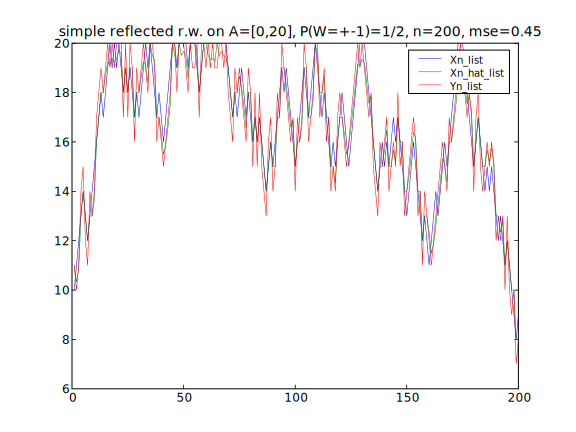
\includegraphics[width=1\textwidth]{hw5_1_K_20_L_1_n_200.eps}
\caption{}
\end{figure}

\begin{figure}[p]
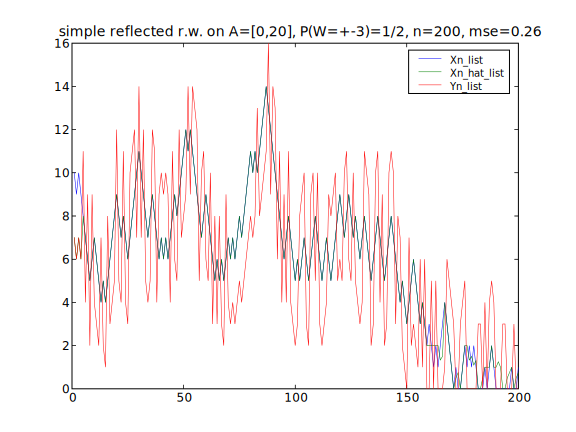
\includegraphics[width=1\textwidth]{hw5_1_K_20_L_3_n_200.eps}
\caption{}
\end{figure}

\begin{figure}[p]
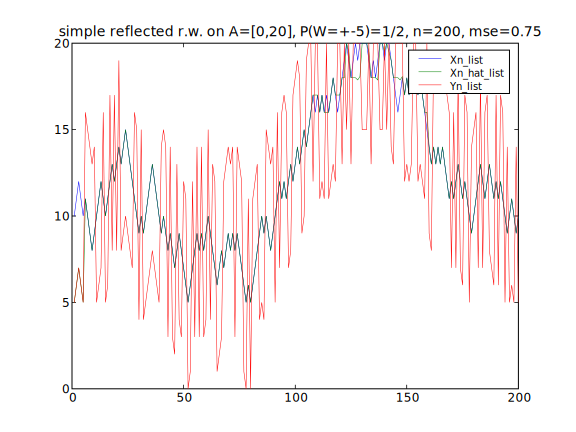
\includegraphics[width=1\textwidth]{hw5_1_K_20_L_5_n_200.eps}
\caption{}
\end{figure}

\begin{figure}
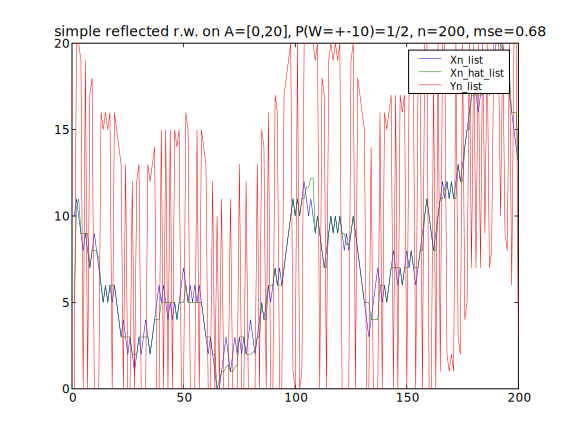
\includegraphics[width=1\textwidth]{hw5_1_K_20_L_10_n_200.eps}
\caption{}
\end{figure}

\begin{figure}
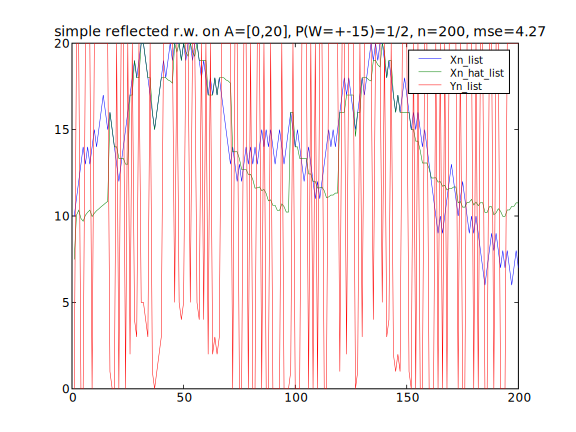
\includegraphics[width=1\textwidth]{hw5_1_K_20_L_15_n_200.eps}
\caption{}
\end{figure}

\begin{figure}
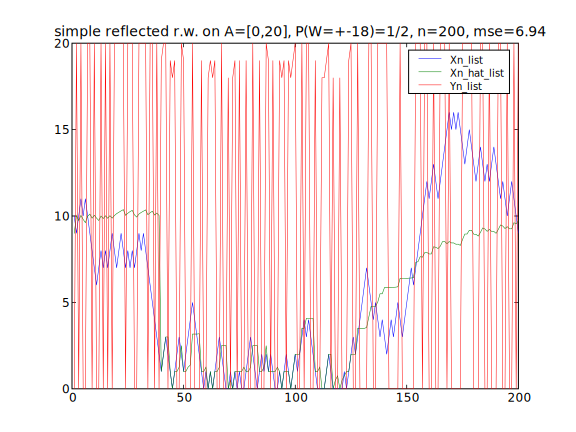
\includegraphics[width=1\textwidth]{hw5_1_K_20_L_18_n_200.eps}
\caption{}
\end{figure}

\begin{figure}
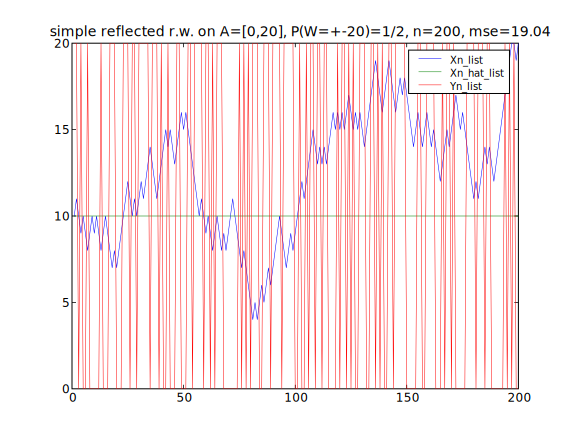
\includegraphics[width=1\textwidth]{hw5_1_K_20_L_20_n_200.eps}
\caption{}
\end{figure}

\section{No. 2}
Tossing of a constant coin with initial coin randomly(uniformly) selected. Given $Y_{[0,4]} = (H, H, H, T, T)$, the $\phi^a_n$ matrix (row is n, column is the hidden state) is

\begin{verbatim}
[[ 0.1         0.16666667  0.23333333]
 [ 0.03        0.08333333  0.16333333]
 [ 0.009       0.04166667  0.11433333]
 [ 0.0063      0.02083333  0.0343    ]
 [ 0.00441     0.01041667  0.01029   ]]
\end{verbatim}

the posterior $\pi^a_n$ matrix is
\begin{verbatim}
[[ 0.2         0.33333333  0.46666667]
 [ 0.10843373  0.30120482  0.59036145]
 [ 0.05454545  0.25252525  0.69292929]
 [ 0.10255019  0.339121    0.55832881]
 [ 0.17558062  0.41473125  0.40968812]]
\end{verbatim}

The estimated $\hat{X_n}$ vector (the state space is $\{0,1,2\}$ is
\begin{verbatim}
[1.266, 1.482, 1.638, 1.456, 1.234]
\end{verbatim}

So it's pretty much the 2nd or 3rd coin.

\end{document}
